% ***********************************************************************************
% Pure LaTeX part to be inserted in a document (be careful of depencies of packages & commands
% Prepared by XXX and YYY under the supervision of Arnaud de La Fortelle
% Fall 2017
% 2D wave propagation subsection of the modeling part
% ***********************************************************************************

\subgroup{2}{Ruitong Zhu and Qingan Zhao}

\paragraph{Model presentation}
This part is to simulate the vibrating string (i.e., 1D wave equation) and present its displacement with a time-varying image. The string held stationary at both ends and free to vibrate transversely subject only to the restoring forces due to tension in the string. $Figure 1$ shows coordinates and definies symbols for the transverse vibrating string. 

\begin{figure}[htb]
	\centering
	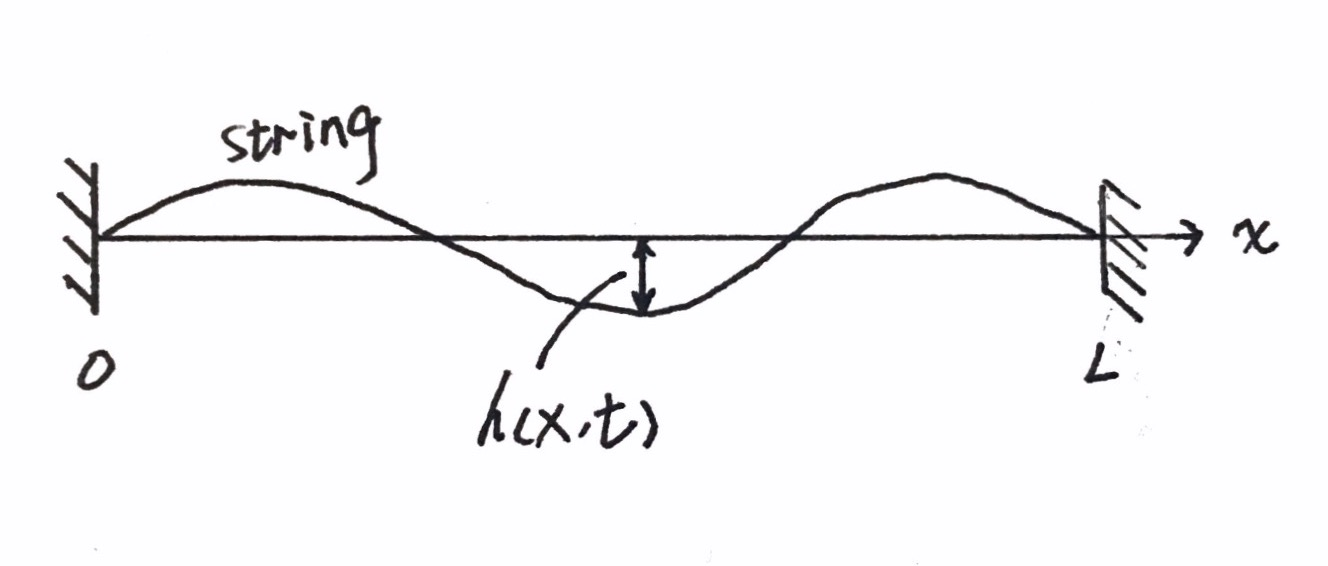
\includegraphics[width=10cm]{string.jpg}       
	\caption{Vibrating String}
\end{figure}

The partial differential equation (PDE) of this problem is given as follow:

\begin{equation}
	\frac{\partial^2 h}{\partial t^2}=a^2\left(\frac{\partial^2 h}{\partial x^2}\right)
\end{equation}

where $h$ is the wave function $h(x,t)$, representing the displacement of the string at position $x$ and time $t$; $a$ is the wave speed which equals to $\sqrt{E/\rho}$.

\paragraph{Implementation}

The simluation is based on Finite Difference Method (FDM). Using second-order central difference at time $t_n$ and position $x_i$, we can get the recurrence equation as follow:

\begin{equation}
\frac{u_{i}^{N+1}-2u_{i}^{N}+u_{i}^{N-1}}{\Delta t^2} = a^2\frac{u_{i+1}^{N}-2u_{i}^{N}+u_{i-1}^{N}}{\Delta x^2}
\end{equation}

Assume the wave speed $a = 1$; the length of the string $L$ is $2$; the maxium time for this simulation is $4$; stepsize $\Delta x$ and $\Delta t$ are both equal to $0.01$. The initial condition and the boundary condition are described as follows:
\begin{eqnarray}
h(x,0)&=&sin(\pi x)\\
\frac{\partial h}{\partial t}\bigg |_{(x,0)}&=&0\\
h(0,t)&=&h(2,t)=0
\end{eqnarray}

Here we offer the implementation in Python:

\begin{python}
	## parameter
	a = 1  ## a coefficient of stiffness
	L = 2  ## The string is constrained at x=0 and x=L.
	T = 4  ## maxium time for this simulation.
	dx = 0.01  ## time step
	dt = 0.01  ## distance step
	N = int(L/dx);
	M = int(T/dt);
	r = (a*dt/dx)**2  ## a parameter

	## initial shape of the string
	def initial(x):
	tmp = math.sin(math.pi*x)
	return tmp
	
	## initial speed of the string
	def speed(x):
	tmp = 0
	return tmp
	
	## Define an array and a blank matrix for later use.
	x = [0]
	h = np.zeros((M+1, N+1))
	
	## t=0, initial condition
	for i in range(N):
	x.append(x[i] + dx)  ## x axis
	h[0,i+1] = initial(x[i+1])  ## displacement of the string
	
	## t=dt, the first itertaion
	for i in range(N-1):
	h[1,i+1] = h[0,i+1] + r* (h[0,i] + h[0,i+2] - 2*h[0,i+1])/2 + dx*speed(x[i+1])
	## displacement of the string
	
	## t=n*dt where n>1
	for j in range(1, M):
	for i in range(N-1):
	h[j+1,i+1] = (h[j,i+2]+h[j,i]-2*h[j,i+1])*r-h[j-1,i+1]+2*h[j,i+1]
	## displacement of the string
	
	t = [0]
	for j in range(M):
	t.append(t[j] + dt)  ## t axis
	
	## Plot the 3D figure.
	fig = plt.figure()
	ax = Axes3D(fig)
	X, T= np.meshgrid(x,t)
	ax.plot_surface(X, T, h, cmap='rainbow')
	ax.set_xlabel('X')
	ax.set_ylabel('T')
	ax.set_zlabel('h')
	plt.show()
	
	## Plot the shape of string at different time
	for i in range(4):
	plt.xlabel(u'x',fontsize=14)
	plt.ylabel(u'h',fontsize=14)
	plt.show()
\end{python}

\paragraph{Results}

The dynamic change of the string is shown in $Figure 2$, ranging from $0\sim 4$.

\begin{figure}[htb]
	\centering
	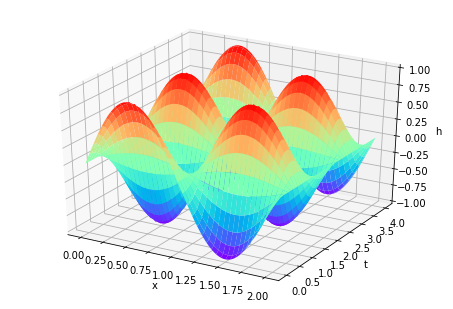
\includegraphics[width=10cm]{string3d.png}       
	\caption{Time-varying Image of the string}
\end{figure}

More specifically, the shapes of the string at different times are shown below:

\begin{figure}[ht]
	\centering
	\begin{minipage}{8cm}
		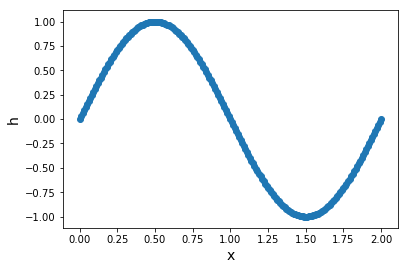
\includegraphics[width=7cm]{string0.png}   
		\caption*{t=0}
		\end{minipage}    
	\begin{minipage}{8cm}
		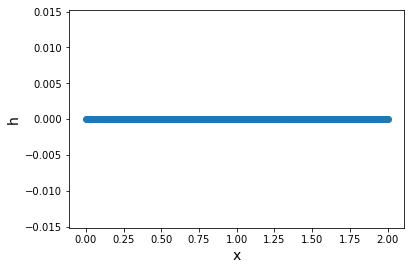
\includegraphics[width=7cm]{string0_5.png}   
		\caption*{t=0.5}
	\end{minipage}  

    \begin{minipage}{8cm}
    	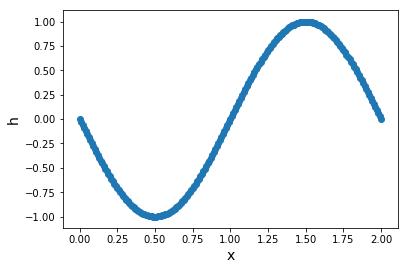
\includegraphics[width=7cm]{string1.png}   
    	\caption*{t=1}
        \end{minipage}  
    \begin{minipage}{8cm}
    	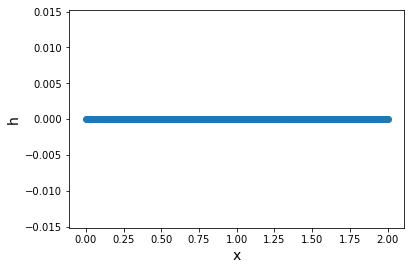
\includegraphics[width=7cm]{string1_5.png}  
    	\caption*{t=1.5} 
    \end{minipage}  
	\caption{Shape of the string at time t}
\end{figure}



\paragraph{Interpretation}

The results are consistent with our expectation. The shape of the string depends on the initial and boundary conditions. In this case, the string is in the shape of a sine wave that changes periodically. 

The initial and boundary conditions can be changed easily at the code by modifying the function $initial()$ and $speed()$. Readers can plot more complicated image with different initial displacement and speed function.

\paragraph{Conclusion}
Finite Difference Method is a practical method to obtain the numerical solution of a Partial Differential Equation. We can learn that it is applicable for one dimentional problems like 1D wave equation and 1D heat equation. It's not difficult to understand but there are some places worth special attention while writing the code. For example, the first iteration needs to be distinguished from other iterations since $t_{N-1}$ is not defined. 

